%!TEX root = ../main.tex

\chapter{Evaluation}
\label{sec:eva}
We have conducted experiments on a Linux machine with 80 cores and 500GB RAM to examine our system RuLES. In this section we report the results of our experimental evaluation, which focuses on 
\emph{(i)} the benefits of our hybrid embedding-based rule quality measure over traditional rule measures; 
\emph{(ii)} the effectiveness of RuLES against the state-of-art Horn rule learning systems; and 
\emph{(iii)} the quality of non-monotonic rules learned by RuLES compared to existing methods.

\section{Experimental Setup}
\label{sec:exper_setup}

\subsection{Datasets}
We performed experiments on the following real world datasets: 

\begin{itemize}
\item \textit{Freebase}: This is a huge knowledge graph consisting of general facts. To meet the requirement of running both rule mining and embedding, we adopt \textit{FB15K} \cite{Bordes:NIPS2013}, a subset of Freebase containing 15K entities, 1345 binary predicates and 592K binary facts, commonly used for evaluating KG embedding models~\cite{DBLP:journals/tkde/WangMWG17}.
\item \textit{Wikidata}: This is a free, community-based knowledge base maintained by the Wikimedia Foundation. In our experiments, we created a subset of Wikidata dump from December 2014 (also used in \cite{amie}) by choosing triples that have entities appearing at least 20 times in the whole dataset, and then selecting top 100 predicates that have most number of facts. This results in a dataset with 250K binary facts over 44K entities and 100 relations, which we refer to as \textit{Wiki44K}.
\item \textit{IMDB}\footnote{\url{http://www.imdb.com/}}: We construct a domain-specific KG from \textit{IMDB} dataset, which is also used in \cite{trantowards}. The KG consists of 118K entities, 37 predicates and 301K binary facts.
\end{itemize}

In the experiments, for each incomplete KG $\cG$, we need its \emph{ideal} completion $\cG^i$ that would give us a gold standard for evaluating our approach and comparing it to others.
Since obtaining a real life $\cG^i$ is hard, we used the KGs \textit{FB15K}, \textit{Wiki44K}, and \textit{IMDB} as reference graphs $\cG^i_{appr}$ that approximate $\cG^i$. 
We then constructed $\cG$ by randomly selecting $80\%$ of its facts while preserving the distribution of facts over predicates. Figure \ref{table:pred_distribution} demonstrates the distribution of facts over top 50 predicates for the 3 datasets.

\begin{figure}[t]
     \centering
     \subfloat[FB15K]{{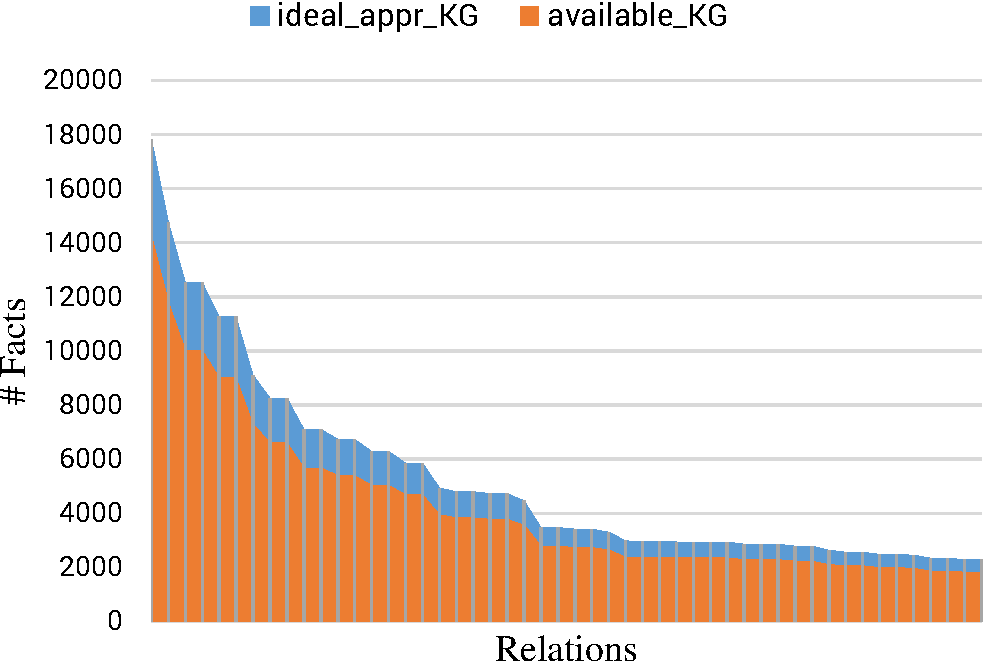
\includegraphics[width=0.5\textwidth]{figures/technical_rp/fb15k_pred_dist-crop.pdf} }}
     \subfloat[Wiki44K]{{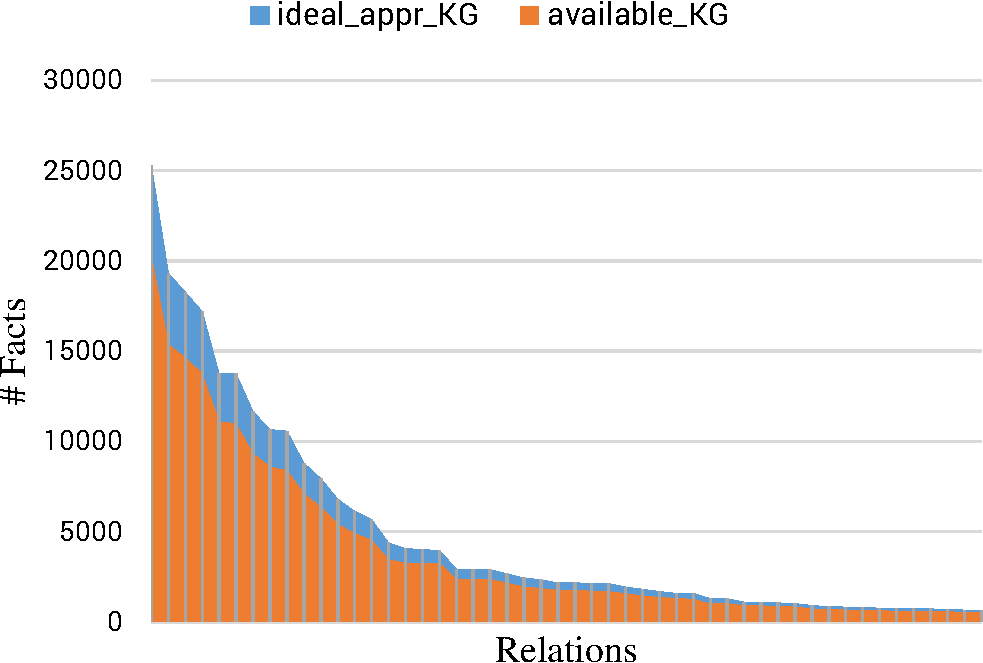
\includegraphics[width=0.5\textwidth]{figures/technical_rp/wiki44k_pred_dist-crop.pdf} }}\\
     \subfloat[IMDB]{{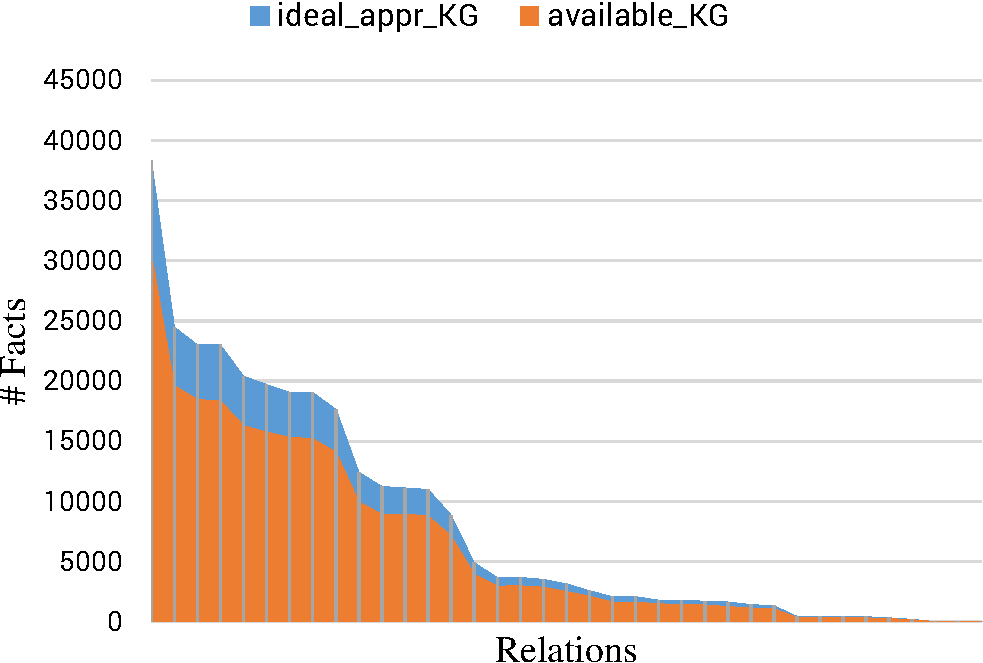
\includegraphics[width=0.5\textwidth]{figures/technical_rp/imdb_pred_dist-crop.pdf} }}
     \caption{Distribution of facts over relations of KGs $\cG^i_{appr}$ and $\cG$.}
     \label{table:pred_distribution}
\end{figure}

\subsection{Embedding Models} 

TransE \cite{Bordes:NIPS2013} and HolE \cite{DBLP:conf/aaai/NickelRP16} are two state-of-the-art embedding models that do not account for external data. In contract, SSP \cite{DBLP:conf/aaai/0005HMZ17} is a state-of-the-art model which accounts for short textual descriptions attached to KG entities. We focus on these 3 embedding models in this work, since they are efficient and relatively simple.
\begin{table}[t]
\centering
\begin{tabular}{|l|r r|r r|r r|r r|r r|r r|} 
 \hline
 DATASET & \multicolumn{4}{|c|}{FB15K} & \multicolumn{4}{|c|}{Wiki44k} & \multicolumn{4}{|c|}{IMDB}\\
 \hline
 MODEL & \multicolumn{2}{|c|}{MRR}& \multicolumn{2}{|c|}{Hits@10(\%)} & \multicolumn{2}{|c|}{MRR}& \multicolumn{2}{|c|}{Hits@10(\%)} & \multicolumn{2}{|c|}{MRR}& \multicolumn{2}{|c|}{Hits@10(\%)} \\
 $Eval.\ setting$ & $Raw$ & $Filt.$ & $Raw$ & $Filt.$ & $Raw$ & $Filt.$ & $Raw$ & $Filt.$ & $Raw$ & $Filt.$ & $Raw$ & $Filt.$\\
 \hline
 TransE& 0.23 & 0.33 & 47.48 & 59.64 & 0.22 & 0.26 & 39.23 & 43.58 & 0.26 & \textbf{0.31} & 36.63 & \textbf{40.39}\\
 HolE & 0.24 & 0.36 & 47.54 & 60.45& 0.14 & 0.18 & 24.54 & 28.38  & 0.21 & 0.26 & 28.27 & 32.08 \\
 SSP & 0.29 & \textbf{0.45}& 55.73 & \textbf{70.35}& 0.26 & \textbf{0.31} & 45.15 & \textbf{51.05} & -- & -- & -- & -- \\
 \hline
\end{tabular}
\caption{Performance of embedding models on the three data sets.}
\label{table:embedding_performance}
\end{table}


We reuse existing implementations of TransE, HolE\footnote{\url{https://github.com/mnick/scikit-kge}}, and SSP\footnote{\url{https://github.com/bookmanhan/Embedding}} and trained these embedding models on the available KGs until convergence using Stochastic Gradient Descent. While we train embedding models on \textit{IMDB} without external text, these embedding models are trained on \textit{FB15K} and \textit{Wiki44K} with 2 different settings: with and without the external textual data. In particular, each entity of \textit{FB15K} and \textit{Wiki44K} links to a small piece of description text, which is extracted from the corresponding Wikidata page. Furthermore, we discard all entities having empty description text for both experimental settings.

For evaluation protocol of the embedding models, we followed the same method of HolE \cite{DBLP:conf/aaai/NickelRP16}. To validate and test the models, we sampled 2000 facts from $\cG^i_{appr} \setminus \cG$ into the validation set, and other 2000 facts into the test set. We report the Mean Reciprocal Rank and the percentage of Hit@10 in Table \ref{table:embedding_performance}. The optimal hyperparameters  of each model and dataset are computed via grid search. We select the hyperparameters, which result in the highest MRR score with \textit{filtered} setting on the validation set. We refer to \cite{DBLP:conf/aaai/NickelRP16} for details.

According to Table \ref{table:embedding_performance}, we compared the effectiveness of the models and selected for each KG the best one. Apart from SSP, which showed the best performance on both FB15K and Wiki44K, we also selected HolE for FB15K and TransE for Wiki44K and IMDB. Note that in this work as a proof of concept we considered some of the most popular embedding models, but conceptually any model (see \cite{DBLP:journals/tkde/WangMWG17} for overview) can be used in our system.

\subsection{Evaluation Metrics} 
To evaluate the learned rules we use the quality of predictions that they produce %through applying the 
when applied on $\cG$, i.e., the more correct facts beyond $\cG$ a ruleset produces, the better it is.  
We consider two evaluation settings: \emph{closed world} setting (CW) and \emph{open world} setting (OW). 
In the CW setting, we define the prediction precision of a rule $r$ and a set of rules $R$ as:
\begin{align*}
  pred\_prec_{CW}(r) = \frac{|\cG_r \cap \cG^i_{appr} \setminus \cG|}{|\cG_r \setminus \cG|},
  \quad 
  pred\_prec_{CW}(R) = \frac{\sum\limits_{r\in R} pred\_prec_{CW}(r)}{|R|}
\end{align*}  
In the OW setting, we also take into account the incompleteness of $\cG^i_{\mi{appr}}$ and  
consider the quality of predictions outside it by performing a random sampling and manually annotating the sampled facts relying on Web resources such as Wikipedia. Thus, we define the OW prediction precision $\mi{pred\_prec_{OW}}$ for a set of rules $R$ as follows:
\[
pred\_prec_{OW}(R) = \frac{|\cG'\cap \cG^i_{\mi{appr}}|+|\cG'\backslash \cG^i_{\mi{appr}}|\times \mi{accuracy(\cG'\backslash \cG^i_{\mi{appr}})}}{|\cG'|}
\]
where $\cG'=\bigcup_{r\in R}\cG_r\backslash \cG$ is the union of predictions generated by rules in $R$, and $\mi{accuracy(S)}$ is the approximated ratio of true facts inside $S$ computed via manual checking of facts sampled from $S$. 
Finally, to evaluate the meaningfulness of exceptions in a rule (i.e., negated atoms) we compute the \textit{revision precision}, which according to~\cite{trantowards} is defined as the ratio of incorrect facts in the difference between predictions produced by the Horn part of a rule and its non-monotonic version over the total number of predictions in this difference (the higher the revision precision, the better the rule exceptions) computed per ruleset. Formally,
\begin{align*}
rev\_prec_{OW}(R) = 1-\frac{|\cG'' \cap \cG^i_{\mi{appr}}|+|\cG''\backslash \cG^i_{\mi{appr}}|\times \mi{accuracy(\cG''\backslash \cG^i_{\mi{appr}})}}{|\cG''|}  
\end{align*}
where $\cG''=\cG_H\backslash \cG_R$ and $H$ is the set of Horn parts of rules in $R$. 
Intuitively, $\cG''$ contains facts not predicted by the rules in $R$ but predicted by their Horn versions. 
 
\subsection{RuLES Configuration}
We run RuLES in several configurations where $\mu_1$ is set to either \textit{standard confidence (Conf)} or \textit{PCA confidence (PCA)}. Furthermore, while we require $\mu_1 \in [0,1]$, we also consider $non\text{-}[0,1]$ metrics, which does not hold this condition, to realize $\mu_1$ (e.g. $conviction$). Meanwhile, $\mu_2$ is computed based on either TransE, HolE, or SSP models.
Throughout the experiments, the configurations are named as \textbf{$\mu_1$-$\mu_2$} (e.g. Conf-HolE). 

\section{Embedding-Based Hybrid Quality Function}
\begin{figure}[t]
     \centering
     \subfloat[Conf-HoLE on FB15K]{{\includegraphics[width=0.5\textwidth]{figures/technical_rp/fb15k_hole_conf-crop.pdf} }\label{fig:fb-conf-hole}}
     \subfloat[Conf-SSP on FB15K]{{\includegraphics[width=0.5\textwidth]{figures/technical_rp/fb15k_ssp_conf-crop.pdf}}\label{fig:fb-conf-ssp}}\\
     \subfloat[PCA-HolE on FB15K]{{\includegraphics[width=0.5\textwidth]{figures/technical_rp/fb15k_hole_pca-crop.pdf} }}
     \subfloat[PCA-SSP on FB15K]{{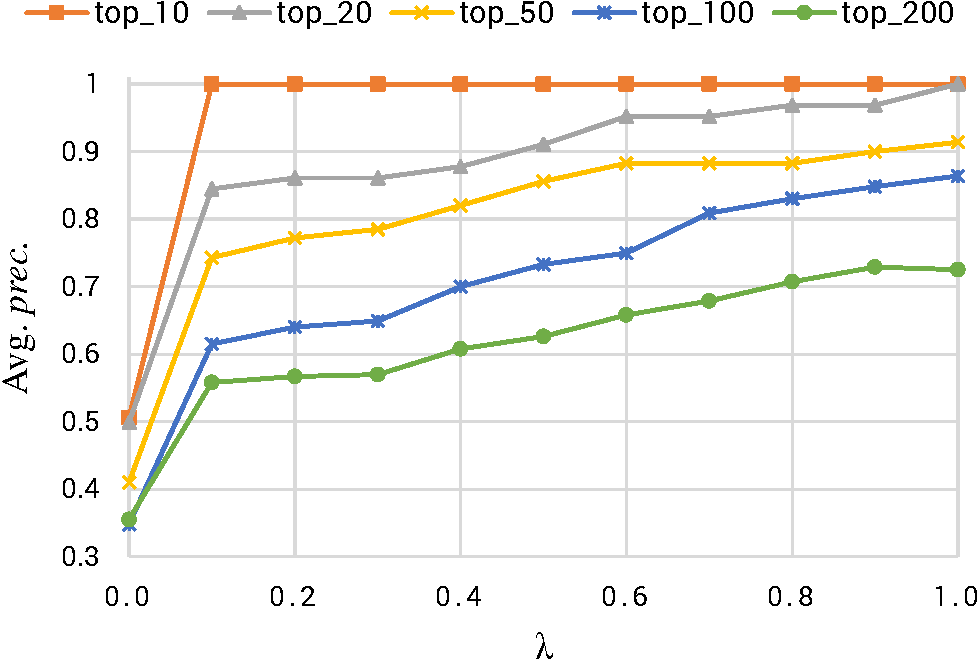
\includegraphics[width=0.5\textwidth]{figures/technical_rp/fb15k_ssp_pca-crop.pdf} }} \\   
     \subfloat[Conv-HolE on FB15K]{{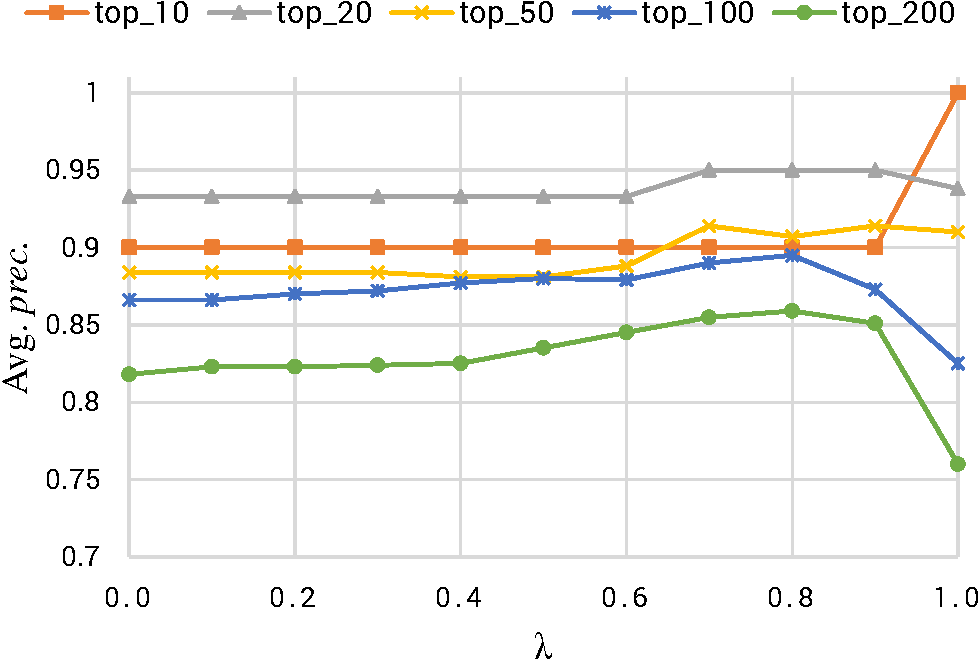
\includegraphics[width=0.5\textwidth]{figures/technical_rp/fb15k_hole_conv-crop.pdf} }}
     \subfloat[Conv-SSP on FB15K]{{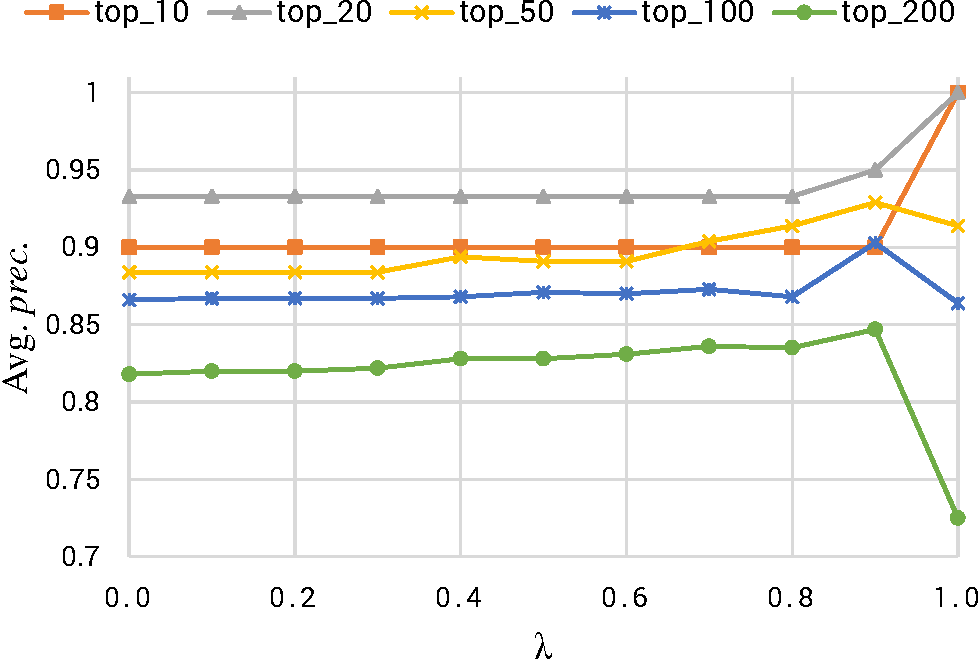
\includegraphics[width=0.5\textwidth]{figures/technical_rp/fb15k_ssp_conv-crop.pdf} }} \\   
     \caption{Avg. prediction precision of the \textit{top-k} rules with various \textit{embedding weights} on FB15K dataset.}
     \label{fig:appendix_exp1_fb15k}
\end{figure} 
\begin{figure}[t]
     \centering
     \subfloat[Conf-TransE on Wiki44K]{{\includegraphics[width=0.5\textwidth]{figures/technical_rp/wiki44k_transe_conf-crop.pdf}}\label{fig:wiki-conf-transe}}
     \subfloat[Conf-SSP on Wiki44K]{{\includegraphics[width=0.5\textwidth]{figures/technical_rp/wiki44k_ssp_conf-crop.pdf}}\label{fig:wiki-conf-ssp}}\\
     \subfloat[PCA-TransE on Wiki44K]{{\includegraphics[width=0.5\textwidth]{figures/technical_rp/wiki44k_transe_pca-crop.pdf} }}
     \subfloat[PCA-SSP on Wiki44K]{{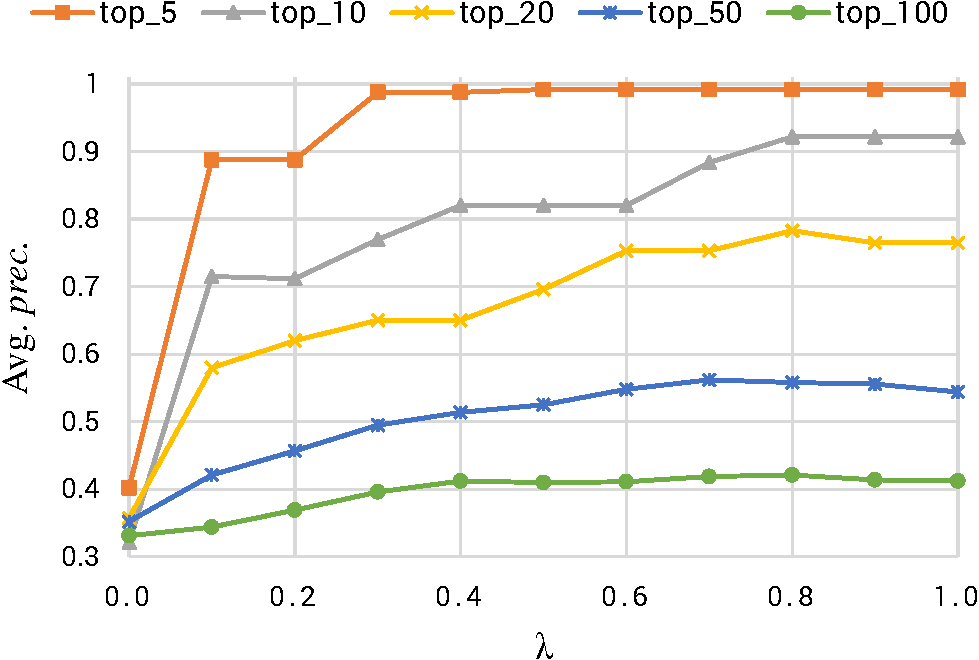
\includegraphics[width=0.5\textwidth]{figures/technical_rp/wiki44k_ssp_pca-crop.pdf} }} \\   
     \subfloat[Conv-TransE on Wiki44K]{{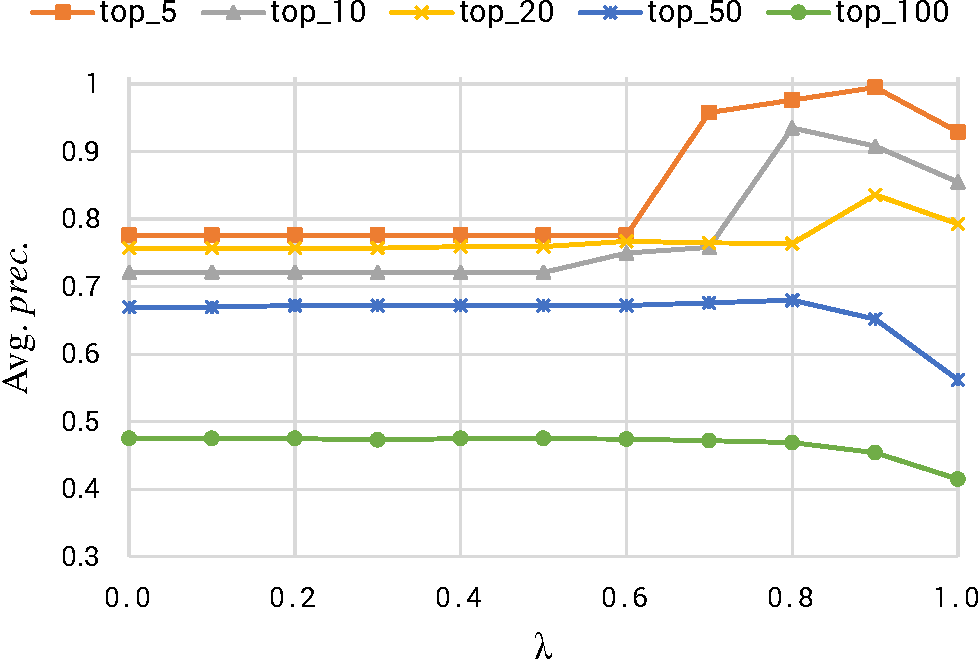
\includegraphics[width=0.5\textwidth]{figures/technical_rp/wiki44k_transe_conv-crop.pdf} }}
     \subfloat[Conv-SSP on Wiki44K]{{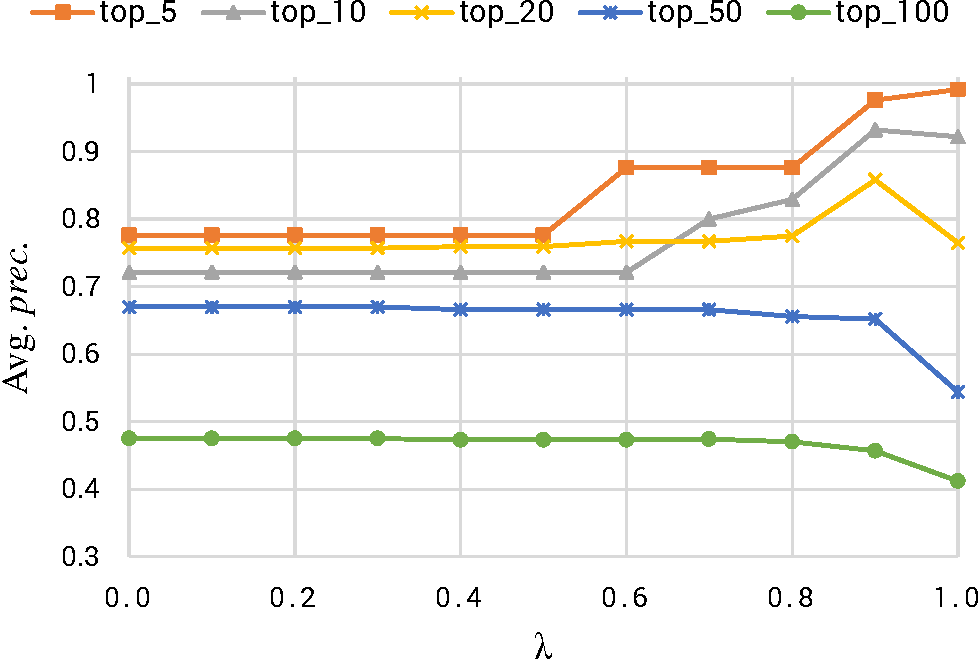
\includegraphics[width=0.5\textwidth]{figures/technical_rp/wiki44k_ssp_conv-crop.pdf} }}\\   
     \caption{Avg. prediction precision of the \textit{top-k} rules with various \textit{embedding weights} on Wiki44K dataset.}
     \label{fig:appendix_exp1_wiki44k}
\end{figure} 

\begin{figure}[t]
     \centering
     \subfloat[Conf-TransE on IMDB]{{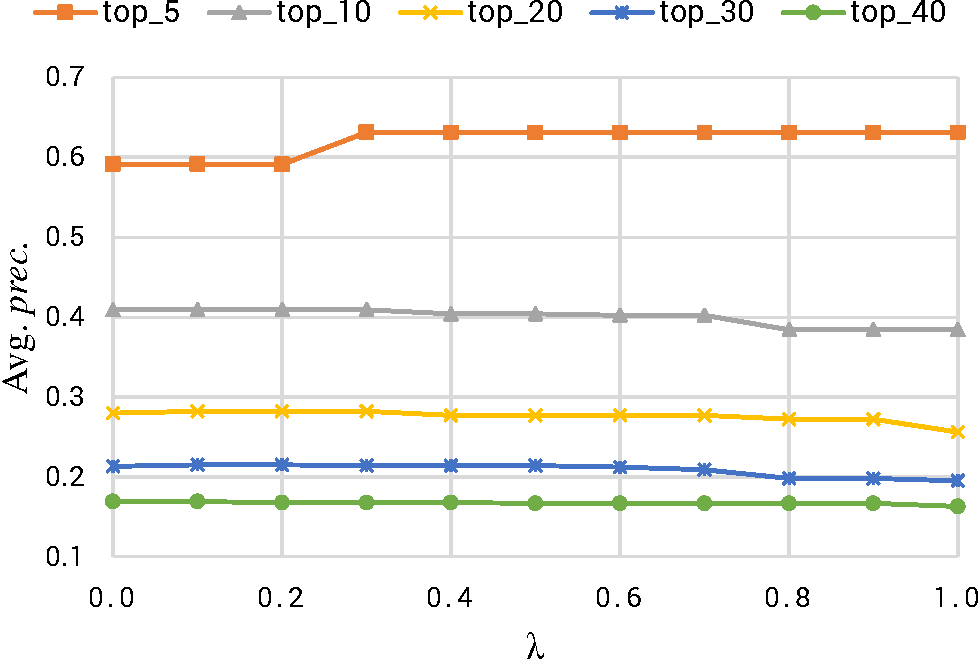
\includegraphics[width=0.5\textwidth]{figures/technical_rp/imdb_transe_conf-crop.pdf} }\label{fig:imdb-conf-transe}}
     \subfloat[PCA-TransE on IMDB]{{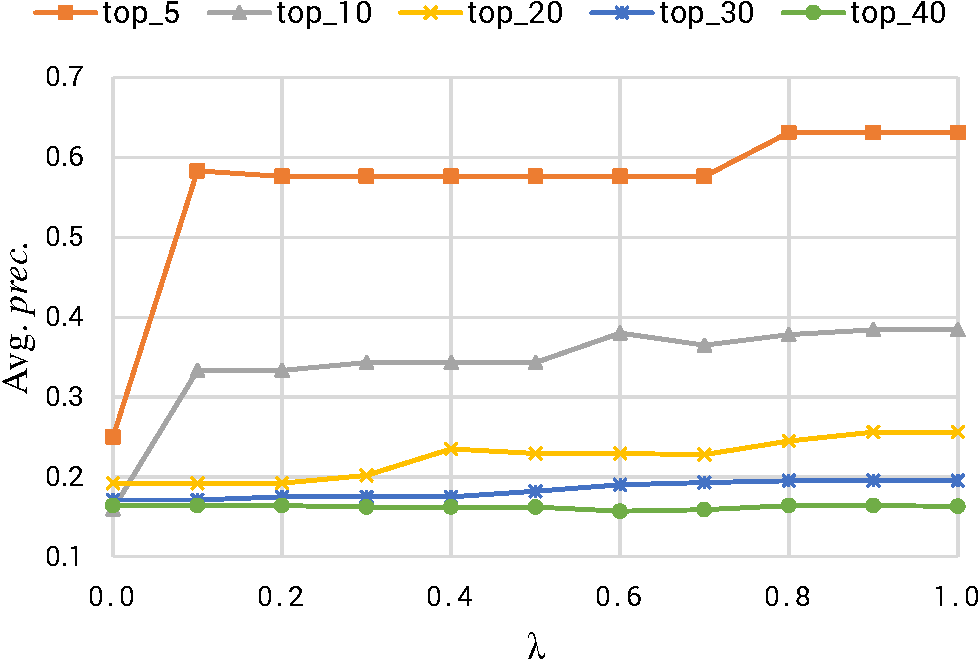
\includegraphics[width=0.5\textwidth]{figures/technical_rp/imdb_transe_pca-crop.pdf} }}\\
     \subfloat[Conv-TransE on IMDB]{{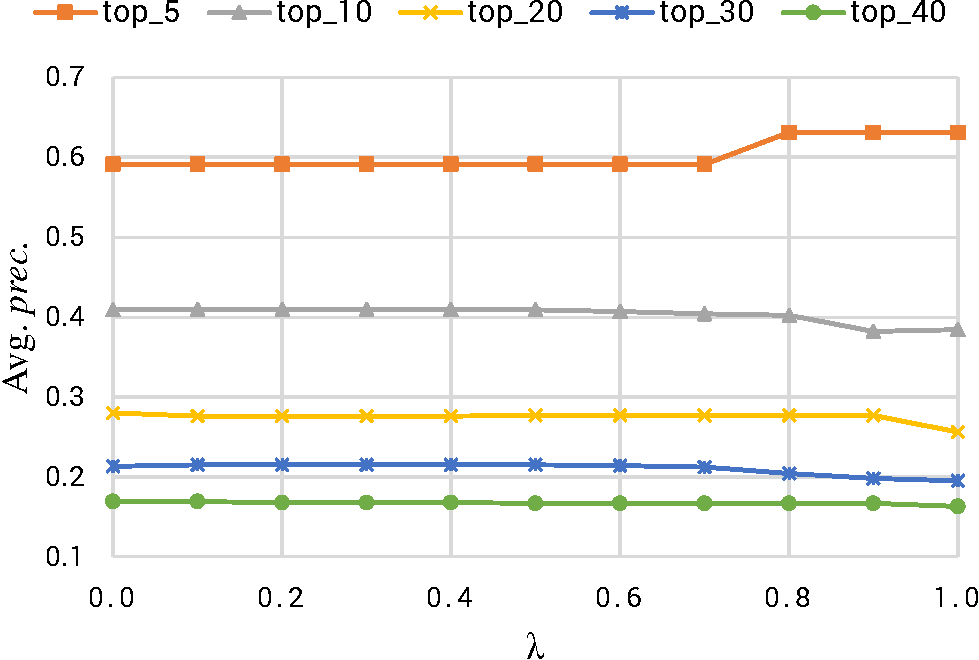
\includegraphics[width=0.5\textwidth]{figures/technical_rp/imdb_transe_conv-crop.pdf} }}     
     \caption{Avg. prediction precision of the \textit{top-k} rules with various \textit{embedding weights} on IMDB dataset.}
     \label{fig:appendix_exp1_imdb}
\end{figure}
\subsection{Hybrid quality function versus standard rule metrics} \label{exp:1}
In this experiment we study the effect of using our hybrid embedding-based 
rule measure $\mu$ from Equation~\ref{eq:hm} on the 
rule ranking compared to traditional measures. 
We do it by first 
learning rules of the form $r:\;h(X,Z) \leftarrow p(X,Y), q(Y,Z)$ from $\cG$ where $\mi{\textit{r-supp}(r,\cG)\geq 10}$, $\mi{conf(r,\cG)\in [0.1,1)}$ and $\mi{\textit{h-cover}(r,\cG)\geq 0.01}$. %at least 
Then, we rank these rules using Equation~\ref{eq:hm} with $\lambda\in \{0, 0.1, 0.2, \dotsc, 1\}$, $\mu_1\in \{\mi{conf,conf_{pca}, conv}\}$ and with $\mu_2$ that is computed by relying on TransE, HolE and SSP.
Note that $\lambda=0$ corresponds to the standard rule measure $\mu_1$ alone.

Figures \ref{fig:appendix_exp1_fb15k}, \ref{fig:appendix_exp1_wiki44k} and \ref{fig:appendix_exp1_imdb} show the %change in the 
average prediction precision $pred\_prec_{CW}$ of the \textit{top-k} rules ranked using our measure $\mu$ for different embedding weights $\lambda$ (\textit{x-axis}). 
In Figures~\ref{fig:fb-conf-hole},~\ref{fig:fb-conf-ssp},~\ref{fig:wiki-conf-transe},~\ref{fig:wiki-conf-ssp} and ~\ref{fig:imdb-conf-transe} %(a,b,d, and e) 
we observe that combining standard confidence ($\mu_1 = conf$)with any %show that combining the confidence with any %other 
%the 
embedding model %results in the increase %rises 
%of 
%in
increases the average prediction precision for %all values of 
%while increasing 
$0\leq \lambda\leq 0.3$. %till it reaches its maximum value around $\lambda=
Moreover, we observe the decrease of prediction precision for $0.4 \leq \lambda\leq 1$ and \textit{top-k} rules learned from FB15K when $k\geq 20$ %starting from \textit{top-20} rules 
and from Wiki44K when $k\geq 10$. %extracted 
%induced from Wiki44K. %\textit{top10}. 
%This behavior is more noticeable . 
This %Hence, it 
shows that the combination of $\mu_1$ and $\mu_2$ gives noticeable positive effect %enhances 
on the prediction results. On the other hand, for $\mu_1=\mi{conf_{pca}}$ the precision increases significantly when combined with embedding models and only decreases slightly %with 
for $\lambda=1$. 
Utilizing $\mi{conf_{pca}}$ instead of $\mi{conf}$ as $\mu_1$ in our hybrid measure is less effective, since 
%The configurations perform worst than standard confidence because 
our training data $\cG$ is randomly sampled %which 
breaking the %local closed world 
partial completeness assumption adopted by the PCA confidence. Meanwhile, with $\mu_1 = conv$, the best value of embedding weight $\lambda$ is close to 1. This is reasonable, since conviction could give us a value greater than 1.

On IMDB dataset, the usage of our hybrid quality measure does improve the quality of result. However, the improvement is not easily noticeable. One explanation is that this dataset is very sparse, which could lead to the ineffectiveness of the embedding models.

\begin{table}[t]
\centering
\begin{tabular}{|c|r r r r r|} 
 \hline
 \multirow{3}{*}{\textbf{\textit{top-k}}} & \multicolumn{5}{|c|}{\textbf{FB15K}}\\
 \cline{2-6}
 & \textbf{{~~~~~}Conf}&  \textbf{{~~~~~}PCA} & \textbf{{~~~~~}Conv} &\textbf{Conf-HolE}& \textbf{Conf-SSP}\\
  & {\scriptsize($\lambda=0$)} & {\scriptsize($\lambda=0$)} & {\scriptsize($\lambda=0$)} & {\scriptsize($\lambda=0.3$)} & {\scriptsize($\lambda=0.3$)}\\
 \hline
\textbf{5} & 0.800 & 0.638 & \textbf{1.000} & \textbf{1.000} & \textbf{1.000}\\
\textbf{10} & 0.900 & 0.506 & 0.900 & \textbf{1.000} & \textbf{1.000}\\
\textbf{20} & 0.900 & 0.499 & 0.933 & 0.950 & \textbf{1.000}\\
\textbf{50} & 0.881 & 0.410 & 0.884 & 0.936 & \textbf{0.937}\\
\textbf{100} & 0.855 & 0.348 & 0.866 & 0.885 & \textbf{0.895}\\
\textbf{200} & 0.842 & 0.355 & 0.818 & 0.870 & \textbf{0.875}\\
 \hline
\end{tabular}
\begin{tabular}{|c|r r r r r|} 
 \hline
 \multirow{3}{*}{\textbf{\textit{top-k}}} & \multicolumn{5}{|c|}{\textbf{Wiki44K}}\\
 \cline{2-6}
 & \textbf{{~~~~~}Conf}&  \textbf{{~~~~~}PCA} & \textbf{{~~~~~}Conv} &\textbf{{~}Conf-Tr.E}& \textbf{Conf-SSP}\\
  & {\scriptsize($\lambda=0$)} & {\scriptsize($\lambda=0$)} & {\scriptsize($\lambda=0$)} & {\scriptsize($\lambda=0.3$)} & {\scriptsize($\lambda=0.3$)}\\
 \hline
 \textbf{5} & 0.800 & 0.402 & 0.776 & \textbf{0.995} & 0.968 \\
\textbf{10} & 0.638 & 0.321 & 0.721 & 0.863 & \textbf{0.932} \\
\textbf{20} & 0.712 & 0.357 & 0.757 & 0.802 & \textbf{0.825} \\
\textbf{50} & 0.670 & 0.352 & 0.670 & \textbf{0.675} & 0.674 \\
\textbf{100} & \textbf{0.477} & 0.331 & 0.475 & 0.474 & 0.474\\
 \hline
\end{tabular}
\begin{tabular}{|c|r r r r|} 
 \hline
 \multirow{3}{*}{\textbf{\textit{top-k}}} & \multicolumn{4}{|c|}{\textbf{IMDB}}\\
 \cline{2-5}
 & \textbf{{~~~~~}Conf}&  \textbf{{~~~~~}PCA} & \textbf{{~~~~~}Conv} &\textbf{{~}Conf-Tr.E}\\
  & {\scriptsize($\lambda=0$)} & {\scriptsize($\lambda=0$)} & {\scriptsize($\lambda=0$)} & {\scriptsize($\lambda=0.3$)}\\
 \hline
\textbf{5} & 0.591 & 0.250 & 0.591 & \textbf{0.631} \\
\textbf{10} & \textbf{0.409} & 0.160 & \textbf{0.409} & \textbf{0.409} \\
\textbf{20} & 0.280 & 0.192 & 0.280 & \textbf{0.282} \\
\textbf{30} & 0.213 & 0.171 & 0.213 & \textbf{0.214} \\
\textbf{40} & \textbf{0.169} & 0.164 & \textbf{0.169} & 0.168 \\
 \hline
\end{tabular}
\caption{Avg. prediction precision of the rules learned using different measures.}
\label{table:avg_quality}
\end{table}


Table~\ref{table:avg_quality} compactly summarizes the average prediction precision of \textit{top-k} rules ranked by
the standard rule measures and our $\mu$ for the best value of $\lambda=0.3$ and highlights the effect of using the better embedding model (text-enhanced vs standard).
%The last two columns for every KG report the results of using $\mu_2$ based on a more advanced embedding model. 
On \textit{FB15K} and \textit{Wiki44K}, we observe that the accuracy of a utilized embedding model is naturally propagated to the accuracy of the rules that we obtain using our hybrid ranking measure $\mu$. This demonstrates that the use of a better embedding model positively effects %should lead to 
the quality of learned rules. 

\subsection{Handling rules with low support}
\begin{figure}[t]
     \centering
     \subfloat[FB15K]{{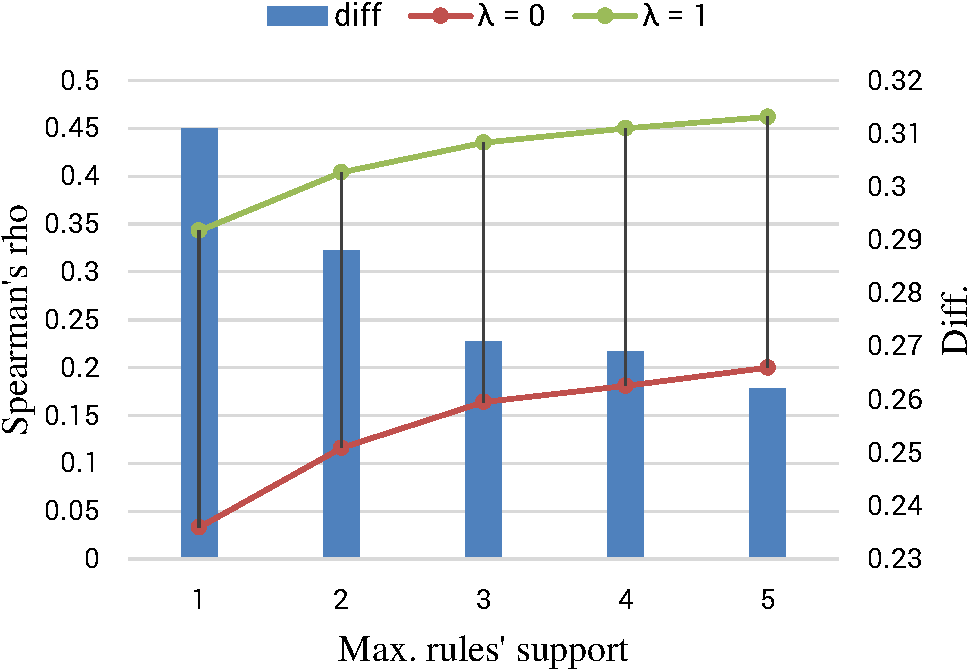
\includegraphics[width=0.5\textwidth]{figures/technical_rp/low_sp_fb15k-crop.pdf} }}
     \subfloat[Wiki44K]{{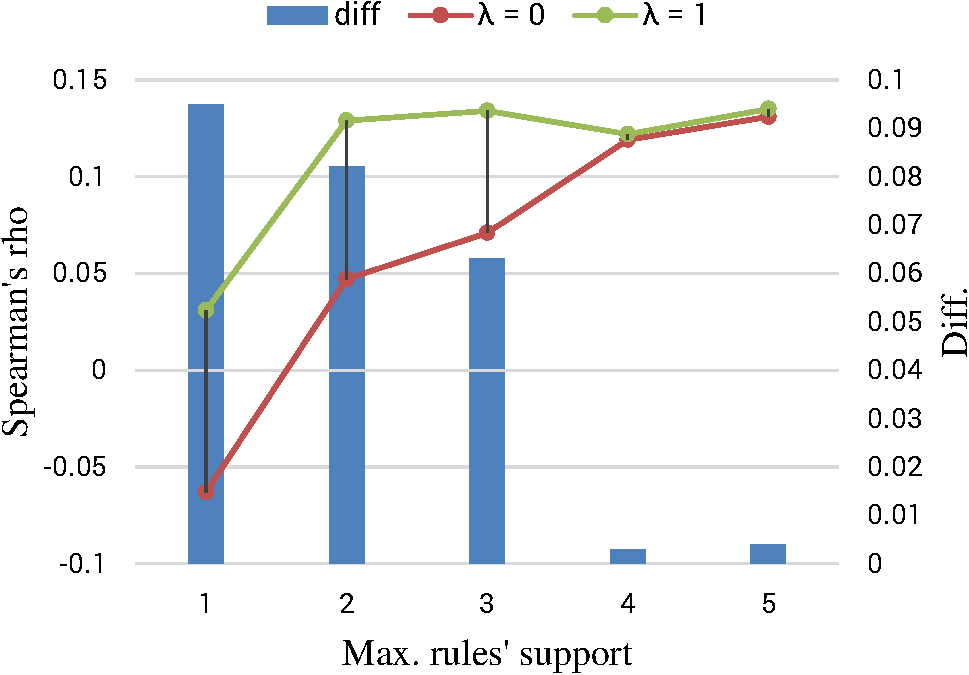
\includegraphics[width=0.5\textwidth]{figures/technical_rp/low_sp_wiki44k-crop.pdf} }}\\
     \subfloat[IMDB]{{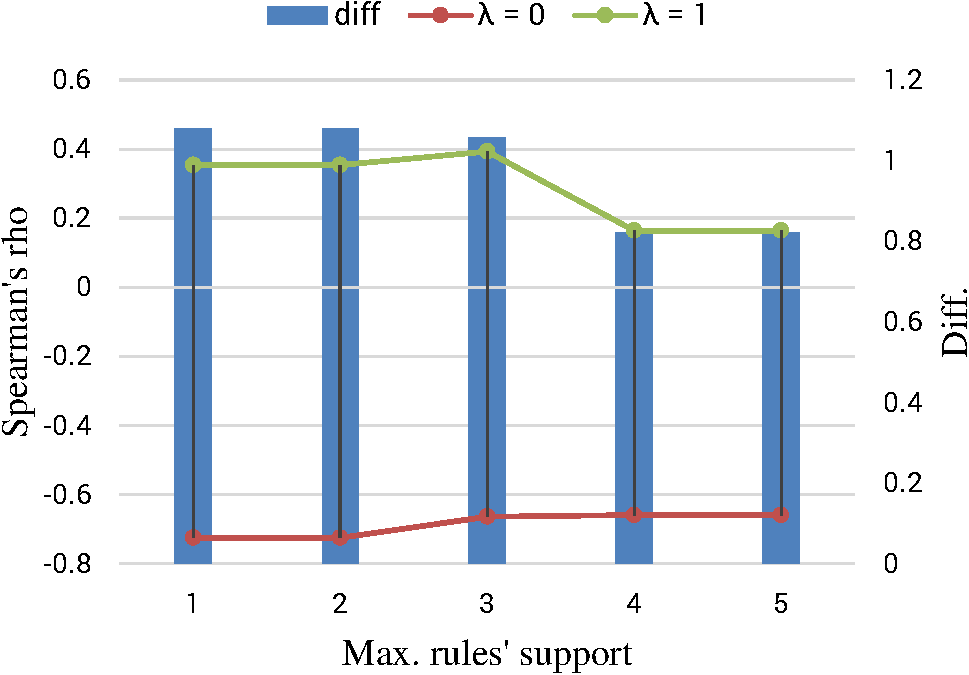
\includegraphics[width=0.5\textwidth]{figures/technical_rp/low_sp_imdb-crop.pdf} }}
     \caption{Spearman's rho of top rules ranked by confidence and the hybrid quality function, with limit on rules' support.}
     \label{fig:low_sp}
\end{figure}
Our hybrid quality function is especially beneficial for assessing rules with low support. Indeed, standard confidence is unreliable for such rules, as it estimates rules' quality by relying only on a small number of rules' instantiations. For example, ignoring all rules having confidence 1 since they do not infer any new facts, when a rule has support 1, its confidence is never greater than 0.5, even though the predicted facts may be true. 

Hybrid quality function $\mu$ fixes this issues by directly looking at the quality of predicted facts, which is achieved by feedback from the embedding models. We verify this hypothesis on \textit{FB15K}, \textit{Wiki44K} and \textit{IMDB} datasets. We also extract rules of form the $r:\;h(X,Z) \leftarrow p(X,Y), q(Y,Z)$ from $\cG$, with $conf(r,\cG) \geq 0.1$ and $\textit{r-supp}(r,\cG) \leq k$, where $k$ indicates the maximum support of rules to be extracted, we try different values of $k \in \{1,2,3,4,5\}$. These rules are then ranked using standard confidence and our hybrid quality function $\mu$. In addition, since we hypothesize that the confidence does not give strong information about the rules in this case, we use $\mu = \mu_2 (\lambda = 1)$, where the hybrid quality function relies only on feedback from the embedding models. To compute $\mu_2$, we use the best embedding models for each dataset: SSP for \textit{FB15K}, \textit{Wiki44K} and TransE for \textit{IMDB}.

To evaluate the quality of the 2 ranked rule lists, we measure the Spearman's rank correlation coefficient (\textit{Spearman's rho}, i.e. Pearson correlation applied to rank)  of rules' confidence or hybrid quality with their $pred\_prec_{CW}$. Figure \ref{fig:low_sp} shows the Spearman's rho of the 2 ranked lists and the difference between them with different values of rules' support limit $k$. The hybrid quality function outperforms standard confidence on 3 datasets, and the results are more visible for lower-support rules.
\section{Horn Rule Learning}
\label{sec:RuLES_vs_AMIE}
%RuLES verses state-of-art}

In this experiment, we compare the Conf-SSP configuration of RuLES (with embedding weight $\lambda = 0.3$) against the state-of-art Horn rule learning system AMIE. We used the default AMIE-PCA configuration with $\mi{conf_{pca}}$ and %  %Also, given the broken partial completeness $\mi{conf_{pca}}$ requires as shown previously, 
% Moreover, we also used the configuration with \textit{standard confidence}, which we refer to as
AMIE-Conf with $\mi{conf}$ measures respectively. For a fair comparison, we set the two configurations of AMIE and our system  to generate rules with at most three positive atoms in the body and  filtered them based on minimum confidence of $0.1$, head coverage of $0.01$ and rule support of $10$ in case of FB15K and $2$ in case of Wiki44K. We then filtered out all rules with $\mi{conf(r,\cG) = 1}$, as they %cannot not infer any new facts. %For evaluation, we use the OW \textit{prediction precision} $pred\_prec_{OW}(R)$ with a sample of 20 prediction outside $\cG^i_{appr}$.
do not produce any predictions.

\setlength{\tabcolsep}{0.1em}
\begin{table}[t]
\centering
\begin{tabular}{|c|r r|r r|r r|r r|r r|r r|}
 \hline
 \multirow{3}{*}{\textbf{\textit{top-k}}}&\multicolumn{6}{|c|}{\textbf{FB15K}} & \multicolumn{6}{|c|}{\textbf{Wiki44K}}\\
 \cline{2-13}&\multicolumn{2}{|c|}{\textbf{AMIE-PCA}}&\multicolumn{2}{|c|}{\textbf{AMIE-Conf}}&\multicolumn{2}{|c|}{\textbf{RuLES}}&\multicolumn{2}{|c|}{\textbf{AMIE-PCA}}&\multicolumn{2}{|c|}{\textbf{AMIE-Conf}}&\multicolumn{2}{|c|}{\textbf{RuLES}} \\
 & \textit{Facts} & \textit{Prec.} & \textit{Facts} & \textit{Prec.} & \textit{Facts} & \textit{Prec.} &\textit{Facts} & \textit{Prec.} &\textit{Facts} & \textit{Prec.} &\textit{Facts} & \textit{Prec.} \\
 \hline
 \textbf{20} & 1029 & 0.28 & 82 & 0.63 & 44 & 1.00 & 185 & 0.73 & 91 & 0.95 & 3291 & 0.98\\
 \textbf{50} & 1716 & 0.43 & 190 & 0.74 & 186 & 0.92 & 47099 & 0.10 & 3594 & 0.95 & 6154 & 0.88 \\
\textbf{100} & 3085 & 0.65 & 255 & 0.78 & 539 & 0.80 & 56831 & 0.20 & 13870 & 0.83 & 13253 & 0.82 \\
\textbf{200} & 10586 & 0.62 & 1210 & 0.83 & 1205 & 0.88 & 82288 & 0.39 & 19538 & 0.72 & 20408 & 0.73 \\
\textbf{500} & 40050 & 0.51 & 2702 & 0.75 & 7124 & 0.95 & 219264 & 0.35 & 124836 & 0.23 & 128256 & 0.48 \\
 \hline
\end{tabular}
\caption{Prediction precision of the \textit{top-k} rules generated by RuLES and AMIE.}
\label{table:amie_vs_RuLES}
\end{table}
\setlength{\tabcolsep}{0.2em}


\begin{table}[t]
\centering
\begin{tabular}{|c|r r|r r|}
 \hline
 \multirow{3}{*}{\textbf{\textit{top-k}}}&\multicolumn{4}{|c|}{\textbf{Family}}\\
 \cline{2-5}&\multicolumn{2}{|c|}{\textbf{NeuralLP}}&\multicolumn{2}{|c|}{\textbf{Conf-TransE}}\\
 & \textit{Facts} & \textit{Prec.} & \textit{Facts} & \textit{Prec.} \\
 \hline
\textbf{10} & 3709 & 0.72 & 4201 & 0.68 \\
\textbf{20} & 8821 & 0.53 & 6957 & 0.72 \\
\textbf{30} & 11337 & 0.49 & 9368 & 0.71 \\
\textbf{40} & 14662 & 0.46 & 11502 & 0.72 \\
\textbf{50} & 18768 & 0.40 & 14547 & 0.62 \\
 \hline
\end{tabular}
\caption{Prediction precision of the \textit{top-k} rules generated by NeuralLP and RuLES.}
\label{table:neurallp_vs_rules}
%\thi{This is added to compare NeuralLP and RuLES}
\end{table}


Table~\ref{table:amie_vs_RuLES} shows the number of facts (see the \textit{Facts} column) predicted by %for 
the set $R$ of \textit{top-k} rules %generated 
in the described settings %. For each set of predictions produced by the set  $R$ of \textit{top-k} rules 
and their prediction precision $pred\_prec_{OW}(R)$ (see the \textit{Prec.} column). %shows the %OW \textit{prediction precision} 
The size of the random sample 
% computed based on facts 
outside $\cG^i_{appr}$ is 20. % and a sample of 20 predictions outside $\cG^i_{appr}$. 
We can observe that on FB15K, RuLES consistently outperforms both AMIE configurations. The \textit{top-20} rules have the highest precision difference (outperforming AMIE-PCA and AMIE-Conf by $72\%$ and $37\%$ respectively).
% AMIE and AMIE-Conf. 
This is explained by the fact that the hybrid embedding quality penalizes rules with higher number of false predictions. %Also 
%Moreover, f
For Wiki44K, RuLES is capable of achieving better precision in most of the cases. %Moreover, for %in 
Notably, for the \textit{top-20} rules RuLES predicted significantly more facts then competitors yet with a high precision. 

In table~\ref{table:neurallp_vs_rules}, we compare RuLES with the recently developed NeuralLP system~\cite{DBLP:conf/nips/YangYC17}. For this we used the Family dataset offered by the authors\footnote{\url{https://github.com/fanyangxyz/Neural-LP}} %with their software %their system which contains 28K facts %distributed covering 
with 28K facts over 3K entities and 12 relations. %As observed 
Starting from the \textit{top-20} rules RuLES is capable of achieving significantly better precision. For the \textit{top-10} rules the precision of NeuralLP is slightly better, but RuLES predicts many more facts.

%!TEX root = ../main.tex


\begin{table}[t]
\centering
\small
\begin{tabular}{|cl|}
	\hline
	%$r_1:$ & $has\_family(X, Y) \leftarrow has\_child(Z, X), has\_family(Z, Y), \textbf{not}\ has\_mother(X, Z).$\\
$r^1{:}$ & $\mi{nationality(X{,}\, Y)}\, {\leftarrow}\, \mi{graduated\_from(X{,}\, Z)}{,}\, \mi{in\_country(Z{,}\, Y)},
	\textbf{not}\ \mi{research\_uni(Z)}$\\
$r^2{:}$ & $\mi{scriptwriter\_of}(X{,}\, Y)\, {\leftarrow}\, \mi{preceded\_by(X{,}\, Z)}{,}\, \mi{scriptwriter\_of(Z{,}\, Y)},
\textbf{not}\ \mi{tv\_series(Z)}$\\
$r^3{:}$ &$\mi{noble\_family(X{,}\, Y)}\, {\leftarrow}\, \mi{ spouse(X{,}\, Z)}{,}\, \mi{noble\_family(Z{,}\, Y)}{,}\,  \textbf{not}\ \mi{ chinese\_dynasties(Y)}$\\
%$r_3:$ &$\mi{sister(X, Y)} \leftarrow \mi{sister(Y, X)}, \textbf{not}\ \mi{brother(X, Y)}$\\

	\hline
\end{tabular}
\caption{Example rules with exception generated by RuLES.}
\vspace*{-3mm}
\label{figure:examples}
\end{table}


\section{RuLES for Exception-Aware Rule Learning}
%----------------------------------------------------------------%
In this experiment, we aim at evaluating the effectiveness of RuLES %in
for learning exception-aware rules.
First, consider in Table~\ref{figure:examples} examples of such rules learned by RuLES over Wiki44K dataset. 
%While %the rule $r_1$ states that a child has the family name from the paternal side and not from the maternal side, the 
 The first rule $r^1$ says that a person is a citizen of the country where his alma mater is located, unless it is a research institution, %university, 
since most %of 
researchers in universities are foreigners. The second rule $r^2$ states that the scriptwriter of some artistic work is also the scriptwriter of its sequel unless it is a TV series, which actually reflects the common practice of having several screenwriters for different seasons. Additionally, $r^3$ encodes that someone belonged to a %royal 
noble family if his/her %the 
spouse is also from the same noble family, excluding the Chinese dynasties. % noble families.

 %Additionally, $r_3$ captures the common sense rule that for two individuals $x,y$ if $y$ is the sister of $x$, then $x$ should also be sister of $y$ unless $x$ is actually the brother of $y$.

%Besides RuLES we also used in the evaluation 
To quantify the quality of RuLES in learning non-monotonic rules, we compare the Conf-SSP configuration of RuLES (with embedding weight $\lambda = 0.3$) with RUMIS~\cite{trantowards}, which is a non-monotonic rule revision system which finds exceptions by minimizing the conflicts between the induced rules. RUMIS learns rules %in 
of the form %of 
$\mi{r:\;h(X,Z) \leftarrow p(X,Y), q(Y,Z), not\; E}$, where $E$ is either $e(X,Z)$ or $\textit{type}(X,t)$ %(\eg type relation); 
%where 
with $t\in \cC_\cG$.
%thus, f
For a fair comparison we restricted RuLES to learn rules of the same form. %of rules.  
We configured both systems %to learn rules 
%with 
setting the minimum rule support threshold to %$\textit{r-supp}(r,\cG)\geqslant 
$10$ and exception confidence for RuLES to $0.05$. %Also 
%Moreover, %for RuLES, 
%we discard rules having exception confidence $\textit{e-conf}(r,\cG)\leqslant 0.05$. 
To enable the systems to %mine %ing 
learn rules with exceptions of the form %following 
$\textit{type}(X,t)$, we enriched the KGs with \textit{type} information from the original Freebase and Wikidata graphs. %Nevertheless, 
%However, types were only considered in the negated part of the body. % while adding exception atoms. 
%Finally, %we keep 
%rules with more than one negated atom were dropped. %a single negative atom. 


% \begin{table}[t]
% \centering
% \begin{tabular}{|r|r r|r r|r r|r r|}
%  \hline
%  \multirow{3}{*}{$top-k$}&\multicolumn{4}{|c|}{FB15K} & \multicolumn{4}{|c|}{WIKI44K}\\
%  \cline{2-9}&\multicolumn{2}{|c|}{RUMIS}&\multicolumn{2}{|c|}{RuLES}&\multicolumn{2}{|c|}{RUMIS}&\multicolumn{2}{|c|}{RuLES} \\
%  & $Avg.scr.$ & $Avg.inc.$ & $Avg.scr.$ & $Avg.inc.$& $Avg.scr.$ & $Avg.inc.$& $Avg.scr.$ & $Avg.inc.$ \\
%  \hline
%  20 & 0.791 & 0.024 & 1.000 & 0.047 & 0.743 & 0.067 & 0.803 & 0.024 \\
%  50 & 0.826 & 0.015 & 1.000 & 0.045 & 0.609 & 0.054 & 0.701 & 0.026 \\
% 100 & 0.859 & 0.026 & 0.990 & 0.047 & 0.417 & 0.033 & 0.539 & 0.011 \\
% 200 & 0.848 & 0.034 & 0.977 & 0.065 & 0.253 & 0.022 & 0.339 & 0.017 \\
% 500 & 0.745 & 0.043 & 0.958 & 0.079 & -- & -- & -- & -- \\
% \hline
% \end{tabular}
% \caption{Average prediction score of some top non-monotonic rules from RuLES vs RUMIS.}
% \label{table:exception_prediction_result}
% \vspace*{-3mm}
% \end{table}
\begin{table}[t]
\centering
\begin{tabular}{|c|r r|r r|r r|r r|}
 \hline
 \multirow{3}{*}{\textbf{\textit{top-k}}}&\multicolumn{4}{|c|}{\textbf{FB15K}} & \multicolumn{4}{|c|}{\textbf{Wiki44K}}\\
 \cline{2-9}&\multicolumn{2}{|c|}{\textbf{RUMIS}}&\multicolumn{2}{|c|}{\textbf{RuLES}}&\multicolumn{2}{|c|}{\textbf{RUMIS}}&\multicolumn{2}{|c|}{\textbf{RuLES}} \\
 & $Facts$ & $Prec.$ & $Facts$ & $Prec.$& $Facts$ & $Prec.$& $Facts$ & $Prec.$ \\
 \hline
\textbf{20} & 672 & 0.95 & 34 & 0.97 & 5844 & 0.93 & 5640 & 0.93 \\
\textbf{50} & 1797 & 0.94 & 158 & 0.99 & 8585 & 0.83 & 13333 & 0.84 \\
\textbf{100} & 2672 & 0.94 & 434 & 0.99 & 21081 & 0.76 & 25265 & 0.81 \\
\textbf{200} & 4103 & 0.87 & 1155 & 0.96 & 50957 & 0.51 & 43677 & 0.67 \\
\textbf{500} & 13439 & 0.76 & 5466 & 0.90 & -- & -- & -- & -- \\
\hline
\end{tabular}
\caption{Prediction precision for the \textit{top-k} rules learned by RUMIS and RuLES.}
\label{table:exception_prediction_result}
\end{table}
% \begin{table}[t]
% \centering
% \begin{tabular}{|r|r r|r r|}
%  \hline
%  \multirow{2}{*}{$top-k$}&\multicolumn{2}{|c|}{FB15K} & \multicolumn{2}{|c|}{WIKI44K}\\
%  \cline{2-5} & RUMIS & RuLES & RUMIS & RuLES \\
%  \hline
%  10 & 0.850 & 0.868 & 0.300 & 0.637 \\
%  %20 & 0.675 & 0.871 & 0.175 & 0.514 \\
%  50 & 0.490 & 0.814 & 0.204 & 0.421 \\
% 100 & 0.590 & 0.785 & 0.124 & 0.271 \\
% 200 & 0.608 & 0.762 & -- & -- \\
% \hline
% \end{tabular}
% \caption{Average revision score of some top rules from RuLES vs RUMIS.}
% \label{table:exception_revision_result}
% \end{table}
\begin{table}[t]
\centering
\begin{tabular}{|r|r r|r r|r r|r r|}
 \hline
 \multirow{3}{*}{\textbf{\textit{top-k}}}&\multicolumn{4}{|c|}{\textbf{FB15K}} & \multicolumn{4}{|c|}{\textbf{Wiki44K}}\\
 \cline{2-9}&\multicolumn{2}{|c|}{\textbf{RUMIS}}&\multicolumn{2}{|c|}{\textbf{RuLES}}&\multicolumn{2}{|c|}{\textbf{RUMIS}}&\multicolumn{2}{|c|}{\textbf{RuLES}} \\
 & $Facts$ & $Prec.$ & $Facts$ & $Prec.$& $Facts$ & $Prec.$& $Facts$ & $Prec.$ \\
 \hline
\textbf{20} & 76 & 0.70 & 111 & 0.68 & 63 & 0.47 & 81 & 0.94 \\
\textbf{50} & 126 & 0.51 & 435 & 0.74 & 191 & 0.28 & 611 & 0.69 \\
\textbf{100} & 183 & 0.43 & 680 & 0.76 & 543 & 0.49 & 1698 & 0.79 \\
\textbf{200} & 310 & 0.30 & 1112 & 0.87 & 4861 & 0.40 & 3175 & 0.80 \\
\textbf{500} & 1155 & 0.53 & 3760 & 0.59 & -- & -- & -- & -- \\
\hline
\end{tabular}
%\caption{Precision of erroneous predictions avoided by rules of RUMIS and RuLES }
\caption{Revision precision for the \textit{top-k} rules learned by RUMIS and RuLES.}
\label{table:exception_revision_result}
\end{table}

%For evaluation, We compute $pred\_prec_{OW}(R)$ for \textit{top-k} rules. 

From the list of mined rules from our system, we keep only rules having some exceptions. If there exist more than 1 such rule having the same positive part, we keep only the one with the highest hybrid quality. In addition, to ensure that the added exception is meaningful, from the list of generated rules from both systems, we keep only rules, whose positive part has standard confidence less than 0.8.

Table~\ref{table:exception_prediction_result} reports the number of predictions produced by a rule set $R$ of %for 
\textit{top-k} non-monotonic rules learned %generated 
by both systems as well as %. For each set $R$ of \textit{top-k} rules, we compute 
their precision $pred\_prec_{OW}(R)$ with a sample of 20 prediction outside $\cG^i_{appr}$. The results show that RuLES consistently outperforms RUMIS %for 
on both datasets. For Wiki44K, and $k\in\{50,100\}$, the \textit{top-k} rules produced by RuLES predicted more facts than those induced by the competitor %as many facts as 
%than RUMIS 
achieving %but with 
higher overall precision. 
Regarding the number of predictions, the converse holds for the FB15K KG; however, the rules learned by RuLES are still more accurate.
%However, in FB15K, the rules generated by RuLES predicted less facts as discussed previously in Section~\ref{sec:RuLES_vs_AMIE}. Note that, the lower the rank of the learned rules, the higher the effect of RuLES in enhancing the prediction quality.

To evaluate the quality of the chosen exceptions, we compare the $rev\_prec_{OW}(R)$ with a sample of 20 predictions. %as explained in Section~\ref{sec:exper_setup}. %As illustrated 
Observe that in Table~\ref{table:exception_revision_result}, rules induced by RuLES prevented the generation of more facts than RUMIS. %those of RUMIS. 
In all of the cases apart from \textit{top-20} for FB15K, our system %RuLES 
managed to remove %achieves higher precision in removing 
a larger fraction of erroneous predictions. %than RUMIS. 
For Wiki44K, RuLES consistently performs twice as good as RUMIS. 
In conclusion, the guidance from the embedding model %using our %hybrid embedding-based quality 
exploited in our system %measure $\mu$ 
%allows us to learn %ing 
%better exception-aware rules, since the feedback from the embedding model 
gives us hints on which among the possible exception candidates likely correspond to noise.   

\section{Summary}
Conducted experiments demonstrate a highly positive impact of the integration of an embedding model on the quality of learned rules. By using an good embedding model, our mining algorithm can extract rules with better predictions' quality, and also capture more meaningful exceptions in comparison with standard methods. 

%  In addition, to see how meaningful the added exception are, table \ref{table:exception_revision_result} reports the precision of removed facts adding exception from some $k$ rules of both systems. The precision of correctly removed facts is also computed by first by looking at $\cG^i_{appr} \setminus \cG$ and second by sampling 20 facts and checking manually ($\cG^i \setminus \cG^i_{appr}$). We can easily notice that our system generates more predictive rules on both datasets in comparison with RUMIS. The reason behind is that RuLES is capable of detecting better exceptions.



%In this experiment, we aim at measuring the quality of our system RuLES on mining exceptions by using the hybrid rule quality scoring function. We use RUMIS \cite{}, which is a state-of-the-art non-monotonic rules mining system, as a baseline to compare our system with. While RUMIS finds exceptions based on only the KG itself, our approach may consider exceptions based on external sources through the embeding models. The setting of the experiment is as follows. We run RUMIS on training KG $\cG$ using the default setting and with OPM ranking method, which is considered its best exception ranking method (see \cite{trantowards}). To reduce running time for RUMIS, we allow only rules with support at least 10. While RUMIS mines only non-monotonic rules with fixed form of the positive part with 3 atoms and support at most 1 exception, our system can generate rules having various forms of positive part, and can even theoretically support more than 1 exception. However, to achieve a fair comparison and reduce the search space, we run our system with the similar setting as RUMIS. In particular, we run our system to generate rules having 3 binary positive atoms and/or 1 additional exception atom. With \textit{exception instantiated atom}, we only allow \textit{\textless rdf:type\textgreater} predicate (i.e. unary predicate), which is the same as in RUMIS. We collect these \textit{\textless rdf:type\textgreater} information for FB15K and Wiki44K from the the whole Freebase and Wikidata dumps, correspondingly. We set the exception coverage of our system to 0.05, minimum rule support also to 10. Other settings regarding selected embedding models, embedding weight and additional filters are similar to the previous experiment. 


%%%%%%%%%%%%%%%%%%%%%%%%%%%% Old text


%% OLD TEXT
%\item \textit{Wikidata} This is a free, community-based knowledge base maintained by the Wikimedia Foundation. In our experiments, we created a subset of Wikidata dump from December 2014 by choosing triples that have entities appearing at least 20 times in the whole dataset, and then selecting top 100 predicates that have most number of facts. We end up with a new dataset with 44k entities, 100 predicates and 250K binary facts. We call this Wiki44K.
%
%% \item \textit{IMDB}\footnote{http://www.imdb.com/} We construct a domain-specific KG from IMDB dataset, which is also used in \cite{Tran2017}. The KG consists of 118K entities, 37 binary predicates, 17K unary predicates and 583K facts (in which, 301K are binary facts).
%\item \textit{Freebase} This is a huge knowledge graph consisting of general facts. To meet the requirement of running both rule mining and embedding, we adopt FB15K \cite{Bordes:NIPS2013}, a dataset containing 15K entities, 1345 binary predicates and 592K binary facts.
%We would like to train the embedding models on the 2 datasets with 2 different settings: with and without the external textual data. In particular, each entity of these datasets is linked with a small piece of description text, which is extracted from the corresponding Wikidata page. Furthermore, we discard all entities having empty description text for both experiments' setting.

%Since obtaining a real life complete ideal KG $\cG^i$ for automatic evaluation is hard, these datasets are used as an approximation $\cG^i_{appr}$ of $\cG^i$. For each dataset, we sample 80\% of facts into the training set (i.e. available graph $\cG$). The rest 20\% will be used for other purposes such as validating or testing.
%% In addition, we ensure that this ratio are equal for each unique predicate. As a side effect, each entity will be connected to at least one other entity.




%%% Old text
%TransE \cite{Bordes:NIPS2013} and HolE \cite{DBLP:conf/aaai/NickelRP16} are two state-of-the-art embedding models regarding the setting of no external data. Meanwhile, when talking about embedding models using additional texts, SSP \cite{DBLP:conf/aaai/0005HMZ17} plays an important part. Apart from prediction quality, these models also have a good running time and memory complexity. Hence, we choose them to evaluate our approach. We reuse the implementation of TransE, HolE from \footnote{https://github.com/mnick/scikit-kge}, and SSP from \footnote{https://github.com/bookmanhan/Embedding}.
%
%We train these embedding models on the available KG $\cG$ of the two datasets Wiki44K and FB15K until convergence using Stochastic Gradient Descent. For evaluation protocol of the embedding models, we use the same method as in TransE \cite{Bordes:NIPS2013} and HolE \cite{DBLP:conf/aaai/NickelRP16}. To validate and test the models, we sampled 2000 facts from the rest 20\% of the dataset (i.e. $\cG^i_{appr} \setminus \cG$) into the validation set, and other 2000 facts into the test set. We report the Mean Reciprocal Rank and the percentage of Hit@10 in table \ref{table:embedding_performance}. The optimal hyperparameters  of each model and dataset are figured out by doing grid search. We select the hyperparameters, which result in the highest MRR score with filtered setting on the validation set. To get a better understanding about how the evaluation is performed, see \cite{Bordes:NIPS2013}.

%\begin{table}[t]
\centering
\begin{tabular}{|l|r r|r r|r r|r r|r r|r r|} 
 \hline
 DATASET & \multicolumn{4}{|c|}{FB15K} & \multicolumn{4}{|c|}{Wiki44k} & \multicolumn{4}{|c|}{IMDB}\\
 \hline
 MODEL & \multicolumn{2}{|c|}{MRR}& \multicolumn{2}{|c|}{Hits@10(\%)} & \multicolumn{2}{|c|}{MRR}& \multicolumn{2}{|c|}{Hits@10(\%)} & \multicolumn{2}{|c|}{MRR}& \multicolumn{2}{|c|}{Hits@10(\%)} \\
 $Eval.\ setting$ & $Raw$ & $Filt.$ & $Raw$ & $Filt.$ & $Raw$ & $Filt.$ & $Raw$ & $Filt.$ & $Raw$ & $Filt.$ & $Raw$ & $Filt.$\\
 \hline
 TransE& 0.23 & 0.33 & 47.48 & 59.64 & 0.22 & 0.26 & 39.23 & 43.58 & 0.26 & \textbf{0.31} & 36.63 & \textbf{40.39}\\
 HolE & 0.24 & 0.36 & 47.54 & 60.45& 0.14 & 0.18 & 24.54 & 28.38  & 0.21 & 0.26 & 28.27 & 32.08 \\
 SSP & 0.29 & \textbf{0.45}& 55.73 & \textbf{70.35}& 0.26 & \textbf{0.31} & 45.15 & \textbf{51.05} & -- & -- & -- & -- \\
 \hline
\end{tabular}
\caption{Performance of embedding models on the three data sets.}
\label{table:embedding_performance}
\end{table}




%First, we focus on comparing our hybrid rule quality scoring function with the two standard rule assessing methods: standard confidence (used by WarmeR) and PCA confidence (used by AMIE). To achieve fair comparison, we only aim at assessing rules having the following form:
%\begin{align*}
%r(X,Z) \leftarrow p(X,Y), q(Y,Z)
%\end{align*}
%Experiment is conducted on both Wiki44K and FB15K datasets. We extract rules of the above form from the training KG $\cG$ that have support at least 10, standard confidence at least 0.1 and head coverage 0.01. All rules with standard confidence 1.0 are also removed, since they do not predict any new facts. These rules are then ordered based on different rule ranking metrics: standard confidence, PCA confidence and our hybrid quality. We computed different versions of hybrid quality, where we use different embedding weights, with standard confidence and PCA confidence as the rule-based metric part. With the setting of no description texts, according to table \ref{table:embedding_performance}, we use TransE for the Wiki44K dataset and HolE for the FB15K dataset, which are the corresponding better models. In addition, we also use SSP model for both datasets. The assessment of these ranking methods are then performed by comparing predictions of these rules on the training set $\cG$ with the approximation $\cG^i_{appr}$. In particular, following \cite{DBLP:conf/semweb/TanonSRMW17}, each rule is given a prediction score, which is computed as the number of predictions inside $\cG^i_{appr} \setminus \cG$ over the number of predictions outside $\cG$:
%\begin{align*}
%    prediction\_score(r) = \frac{|\cG_r \cap \cG^i_{appr} \setminus \cG|}{|\cG_r \setminus \cG_a|}
%\end{align*}
%\captionsetup[subfigure]{textfont=scriptsize}
% \begin{figure}[t]
%    \centering
%    % Gad: to unify legend and save space
%    \subfloat{{\includegraphics[width=0.5\textwidth]{figures/legend.pdf} }}\\[-2ex]
%    \setcounter{subfigure}{0}%
%    \subfloat[Confidence + HolE]{{\includegraphics[width=0.5\textwidth]{figures/fb15k_hole_conf-crop.pdf} }}
%    \subfloat[Confidence + SSP]{{\includegraphics[width=0.5\textwidth]{figures/fb15k_ssp_conf-crop.pdf} }}\\
%    \subfloat[PCA Confidence + HolE]{{\includegraphics[width=0.5\textwidth]{figures/fb15k_hole_pca-crop.pdf} }}
%    \subfloat[PCA Confidence + SSP]{{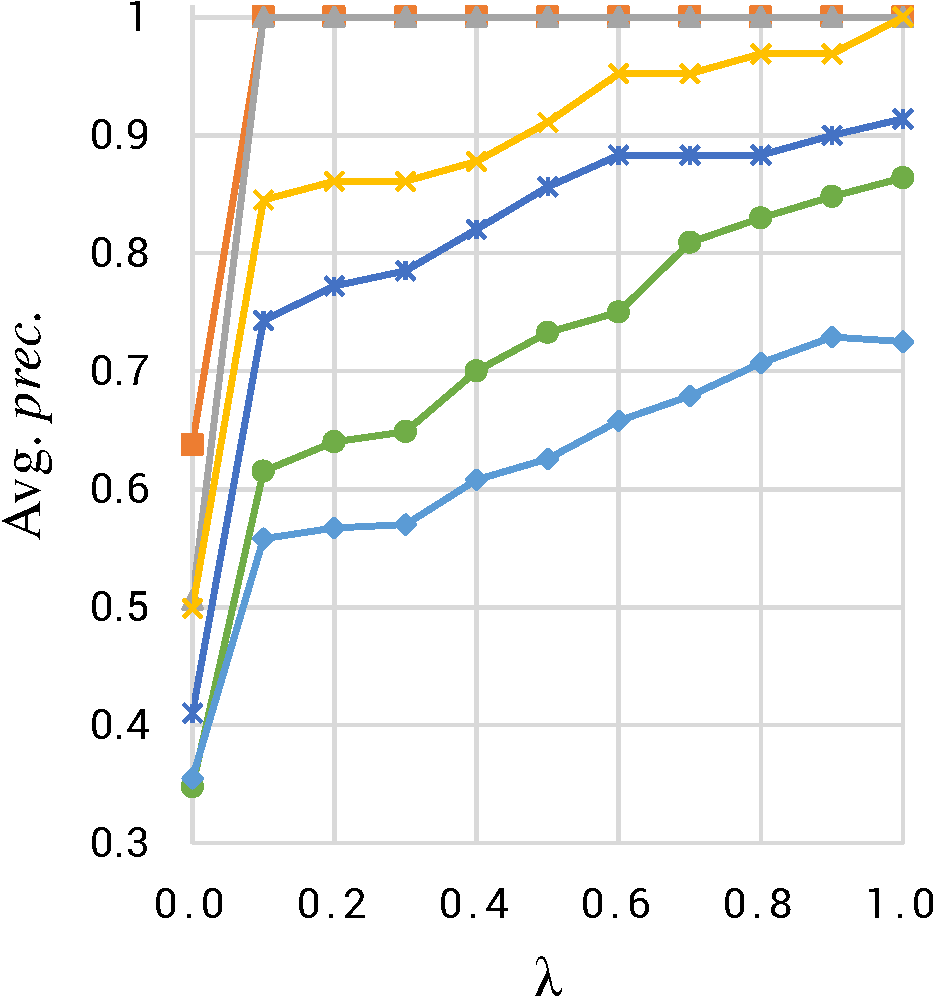
\includegraphics[width=0.5\textwidth]{figures/fb15k_ssp_pca-crop.pdf} }}    
%    \caption{Average prediction score of some top rules on FB15K dataset with the hybrid rule quality scoring function.}
%    \label{fig:fb15k}
% \end{figure}
%
%\begin{figure}[t]
%    \centering
%    \subfloat[Confidence + TransE]{{\includegraphics[width=0.5\textwidth]{figures/wiki44k_transe_conf-crop.pdf} }}
%    \subfloat[Confidence + SSP]{{\includegraphics[width=0.5\textwidth]{figures/wiki44k_ssp_conf-crop.pdf} }}\\
%    \subfloat[PCA Confidence + TransE]{{\includegraphics[width=0.5\textwidth]{figures/wiki44k_transe_pca-crop.pdf} }}
%    \subfloat[PCA Confidence + SSP]{{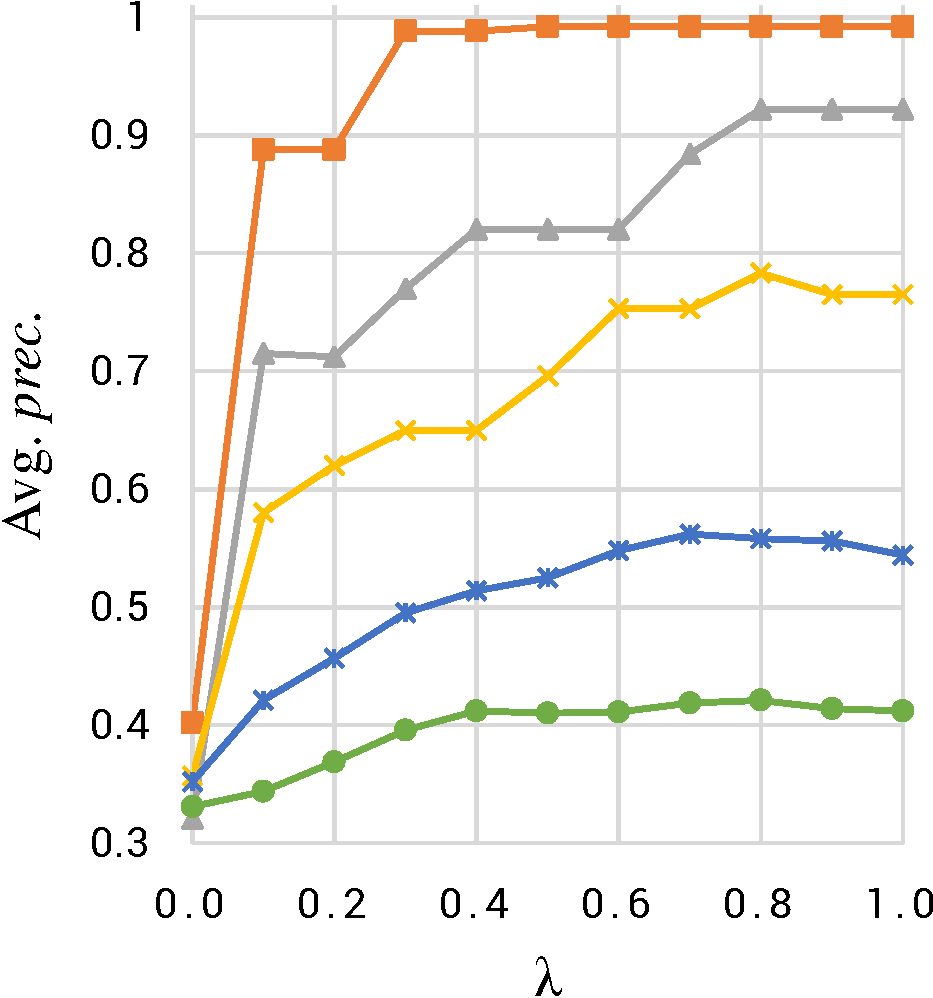
\includegraphics[width=0.5\textwidth]{figures/wiki44k_ssp_pca-crop.pdf} }}    
%    \caption{Average prediction score of some top rules on Wiki44K dataset with the hybrid rule quality scoring function.}
%    \label{fig:wiki44k}
%\end{figure}



%The higher the prediction score is, the better the rule is. Figures \ref{fig:fb15k} and \ref{fig:wiki44k} demonstrate the average prediction score of top $k$ rules on FB15K and Wiki44K datasets when using hybrid quality with different traditional rule-based measures and values of embedding weights $\lambda$. We can see that with each top $k$ rules, their average prediction score rises along with the increasing of parameter $\lambda$ until reaching some optimal value, then falls down until $\lambda$ is equal to 1. Hence, the combination of $q_{rm} $ and $q_{es}$ is crucial to achieve the best result. In addition, the hybrid quality works better than the traditional PCA confidence with every value of $\lambda$. The reason is that our training KG $\cG$ is randomly sampled that break the assumption made by PCA confidence. 











